\title{Лекция 14\\Основные принципы разработки семантических моделей баз знаний}
\author[]{Шункевич Д.В.}
\institute[]{Белорусский государственный университет информатики и радиоэлектроники}

\begin{frame}
	\titlepage
\end{frame}

\begin{frame}{\\Содержание лекции}
	\topline
	\justifying
	Методика разработки баз знаний, основные этапы. Выделение иерархии предметных областей. Формирование онтологий.
\end{frame}

\begin{frame}{Основные этапы разработки баз знаний}
	\topline
	\justifying 
	\begin{SCn}
	\begin{textitemize}
		\item Определение задач системы 
		\item Определение необходимых источников информации
		\item Составление словаря (схемы терминов)
		\item Построение информационного поля
		\item Построение онтологии
		\item Описание экземпляров 
	\end{textitemize}
	\end{SCn}
\end{frame}

\begin{frame}{\\}
	\topline
	\justifying 
	\begin{SCn}
	\scnheader{составление словаря}
	\scnrelfrom{пояснение}{составление неформализованного списка терминов}
	
	\scnheader{построение информационного поля}
	\scnrelfrom{пояснение}{формализация понятий}
	
	\scnheader{построение онтологии}
	\scnrelfrom{пример}{формализация свойств отношений и доменов}
	
	\scnheader{описание экземпляров}
	\scnrelfrom{пояснение}{описание свойств, классов, связей}	
	\end{SCn}
\end{frame}

\begin{frame}{\\Источники информации}
	\topline
	\justifying 
	\begin{SCn}
		\scnheader{источники информации}
		\scnidtf{информационные ресуры}
		\begin{scnrelfromset}{разбиение}
			\scnitem{структурированные}
			\begin{scnindent}
				\scnrelfrom{пример}{диаграмма классов, ER-диаграммы}
			\end{scnindent}
			\scnitem{неструктурированные}
			\begin{scnindent}
				\scnrelfrom{пример}{документ, книга}
			\end{scnindent}
			\scnitem{знания эксперта}
		\end{scnrelfromset}
		\scnheader{структурированный информационный ресурс}
		\scnidtf{информационный ресурс, представленный на языке, синтасис и семантика которого известны}
	\end{SCn}
\end{frame}

\begin{frame}{\\Верификация баз знаний}
	\topline
	\justifying 
	\begin{SCn}
		\scnheader{верификация}
		\scnidtf{проверка}
		
		\scnheader{верифицируемые сущности}
		\begin{scnrelfromset}{разбиение}
			\scnitem {некорректность (ошибочность)}
			\scnitem {неполнота}
			\scnitem {избыточность}
		\end{scnrelfromset}
	\end{SCn}
\end{frame}

\begin{frame}{\\Некорректность}
	\topline
	\justifying 
	\begin{SCn}
		\scnheader{некорректность}
		\scnidtf{существование противоречия между двумя и более фрагментами базы знаний}
		\begin{scnrelfromset}{разбиение}
			\scnitem{противоречие логических формул}
				\begin{scnindent}
					\scnrelfrom{уточнение}{противоречие логических формул в рамках формальной теории}
				\end{scnindent}
			\scnitem{противоречие фактов логических формул}
				\begin{scnindent}
					\begin{scnrelfromset}{разбиение}
						\scnitem{противоречие определений}
						\scnitem{противоречие утверждений}
					\end{scnrelfromset}
				\end{scnindent}
		\end{scnrelfromset}
	\end{SCn}
\end{frame}

\begin{frame}{\\Неполнота}
	\topline
	\justifying 
	\begin{SCn}
		\scnheader{неполнота}
		\scnidtf{противоречие между утверждениями о полноте и фактами из базы знаний системы}
		\scnrelfrom{пояснение}{для каждого понятия можно указать необходимый набор элементов (сущностей), которые будут характеризовать данное понятие}
		\scnrelfrom{пример}{у каждого понятия должен быть индентификатор, предметная область, определение и т.д.}
		\scnrelfrom{пример}{у каждого отношения должен быть домен (домены), арность и т.д.}
	\end{SCn}
\end{frame}

\begin{frame}{\\Избыточность}
	\topline
	\justifying 
	\begin{SCn}
		\scnheader{избыточность}
			\begin{scnrelfromset}{разбиение}
				\scnitem{информационный мусор}
				\scnidtf{данные, которые нужны в контексте решения конкретных задач и после этого не имеют смысла, за исключением ситуации, когда нужно проанализировать процесс решения задачи}
				\scnitem{легковыводимая информация}
			\end{scnrelfromset}
		
	\end{SCn}
\end{frame}

\begin{frame}{\\Легковыводимая информация. Пример}	
	\topline
	\justifying 
	\vspace{10mm}
	\begin{figure}[H]
		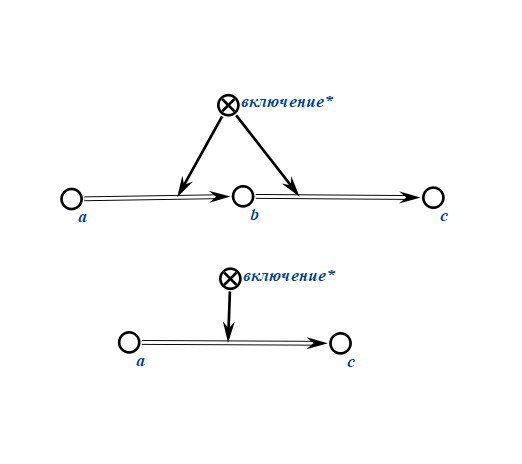
\includegraphics[scale=0.4]{./figures/sd_kb_develop_principles/inclusion.jpeg}
	\end{figure}
\end{frame}

\begin{frame}{\\}
	\topline
	\justifying 
	\begin{SCn}
		Во-первых, использование знаний, которые можно легко вывести (второй пример на предыдущем слайде) из уже имеющихся знаний, экономит память, т.е. не нужно дублировать одно и то же несколько раз.\\
		 \vspace{5mm}
		Во-вторых, избыточность представления знаний (первый пример на предыдущем слайде) позволяет снизить время решения задач, т.е. происходит экономия времени.\\ 
			\vspace{5mm}
		Выбор относительно того, использовать ли избыточное представление знаний или нет, стоит за разработчиком базы знаний.
	\end{SCn}
\end{frame}